\documentclass[runningheads,a4paper]{llncs}

\usepackage{amssymb}
\setcounter{tocdepth}{3}
\usepackage{graphicx}

\usepackage{makeidx}  % allows for indexgeneration
\usepackage{amssymb, amsmath, amsfonts, graphics, graphicx}
\usepackage{enumerate}

\usepackage{longtable}

\usepackage{url}
\urldef{\mailsa}\path|{alfred.hofmann, ursula.barth, ingrid.haas, frank.holzwarth,|
\urldef{\mailsb}\path|anna.kramer, leonie.kunz, christine.reiss, nicole.sator,|
\urldef{\mailsc}\path|erika.siebert-cole, peter.strasser, lncs}@springer.com|
\newcommand{\keywords}[1]{\par\addvspace\baselineskip
\noindent\keywordname\enspace\ignorespaces#1}


%=======================================================================
%==========================DOCUMENT=====================================
%=======================================================================
\begin{document}

\newcommand{\fictAquantor}{\ensuremath{\forall\colon\boldsymbol{True}}}
\newcommand{\fictEquantor}{\ensuremath{\exists\colon\boldsymbol{True}}}
\newcommand{\bomega}{\boldsymbol{\omega}}
\newcommand{\bphi}{\boldsymbol{\phi}}
\newcommand{\eqdef}{\stackrel{\mathrm{df}}{=}}
\newcommand{\bigand}[2]{\raisebox{-4pt}{\ensuremath{\overset{#1}{\underset{#2}{\text{\huge\&\normalfont}}}}}}

\mainmatter  % start of an individual contribution

% first the title is needed
\title{Software for Automated Theorem Proving Based on the Calculus of Positively Constructed Formulas\thanks{Ok}}
% a short form should be given in case it is too long for the running head
\titlerunning{ATP Based on the PCF Calculus}

% the name(s) of the author(s) follow(s) next
%
% NB: Chinese authors should write their first names(s) in front of
% their surnames. This ensures that the names appear correctly in
% the running heads and the author index.
%
\author{Alexander Larionov\and Artem Davydov\and Evgeny Cherkashin}
%
%\authorrunning{Lecture Notes in Computer Science: Authors' Instructions}
% (feature abused for this document to repeat the title also on left hand pages)

% the affiliations are given next; don't give your e-mail address
% unless you accept that it will be published
\institute{Irkutsk State University,
              1, Karl Marks str., Irkutsk, Russia \\
           Institute for System Dynamics and Control Theory at Siberian Branch
              of Russian Academy of Sciences,
              134, Lermontov str., Irkutsk, Russia\\
           Irkutsk National Research Technical University,
              83, Lermontov str., Irkutsk, Russia
%\mailsa\\
%\mailsb\\
%\mailsc\\
%\url{http://www.springer.com/lncs}
}

%
% NB: a more complex sample for affiliations and the mapping to the
% corresponding authors can be found in the file "llncs.dem"
% (search for the string "\mainmatter" where a contribution starts).
% "llncs.dem" accompanies the document class "llncs.cls".
%

\toctitle{Lecture Notes in Computer Science}
\tocauthor{Authors' Instructions}
\maketitle


%=======================================================================
%==========================ABSTRACT=====================================
%=======================================================================
\begin{abstract}
A description of the calculus of positively constructed formulas (PCF) and prover based on this calculus is considered. The PCF calculus has been developed by Russian scientists S.N. Vassiliev and A.K. Zherlov by an evolutionary way in describing and solving control theory problems. This calculus has features, which are applicable in control theory. The described implementation of the prover uses several techniques and strategies to improve prover performance. The prover is being tested by means of solving problems from TPTP library. The usage of implemented inference search strategies is also commented in this paper.
\keywords{positively constructed formulas, automated theorem proving, proof strategies}
\end{abstract}



%=======================================================================
%==========================INTRODUCTION=================================
%=======================================================================
\section{Introduction}

Originally \cite{SNV1990,ICDS2000} the calculus of positively constructed formulas (PCF) was developed by Russian scientists S.N. Vassilyev and A.K. Zherlov by an evolutionary way in describing and solving control theory (CT) problems. In \cite{ICDS2000} the PCF calculus is presented as first-order logical formalism, examples of CT problems described and solved by the PCF calculus (elevator group control, mobile robot action planning and telescope guidance), as well as proof of soundness and completeness.

The PCF calculus is both machine-oriented, and also human-oriented, naturally aimed at solving the problems of dynamic systems control thanks to its features such as follows: unique inference rule and simple scheme of axioms; modifiability of semantics (constructive, monotonic, temporal, etc.) and besides it is possible to construct intuitionistic inferences of some non-Horn formulas; the explicit usage of $\forall$ and $\exists$ quantifiers, the scolemization procedure is not required.

However, in this paper, we will not cover the human--orientability properties of the PCF calculus and its dynamic systems control properties as well.  This and the calculus capabilities in action planning is described in \cite{ICDS2000}.   Here, we deal with the automatic search of a logical inference, i.e., the inference engine capabilities.  In order to estimate the applicability of the PCF calculus for automatic theorem proving we develop a prover program and test it on problems from TPTP library.

%This paper contains a description of the PCF calculus, an implementation of the prover program, and strategies of logical inference used to direct the inference search algorithms. The results of a comparison of the developed prover system with other provers are presented.


%=======================================================================
%==========================BACKGROUND===================================
%=======================================================================
\section{Preliminaries PCF Calculus}

Let's consider a language of first-order logic (FOL) that consists of first-order formulas (FOFs) built out of atomic formulas with $\&, \vee, \neg, \rightarrow, \leftrightarrow$ operators, $\forall$ and $\exists$ quantifier symbols and constants $true$ and $false$.  The concepts of \emph{term}, \emph{atom}, \emph{literal} we define in the usual way.

Let $X = \{x_1,\ldots,x_k\}$ be a set of variables, $A = \{A_1,\ldots,A_m\}$ be a set of atomic formulas, and $F = \{F_1,\ldots,F_n\}$ be a set of FOFs. Then the following formulas $((\forall x_1) \ldots (\forall x_k) (A_1 \& \ldots \& A_m \rightarrow (F_1 \vee \ldots \vee F_n)))$ and $((\exists x_1) \ldots (\exists x_k) (A_1 \& \ldots \& A_m \& (F_1 \& \ldots \& F_n)))$ are denoted as  $\forall_XA\colon F$ and $\exists_XA\colon F$ respectively, keeping in mind that the $\forall$--quantifier corresponds to $\rightarrow F^{\vee}$, where $F^{\vee}$ means disjunction of all formulas from $F$, and $\exists$--quantifier corresponds to $\& F^{\&}$, where $F^{\&}$ means conjunctions of all formulas from $F$.

If $F = \emptyset$, then the formulas have the form $\forall_XA\colon\emptyset \equiv \forall_XA \rightarrow false$ and $\exists_XA\colon\emptyset \equiv \exists_XA \& true$, since the empty disjunction is identical to $false$, whereas the empty conjunction is identical to $true$.  The form $\forall_XA$ and $\exists_XA$ are abbreviations of such formulas.  If $X = \emptyset$, then $\forall A\colon F$ and $\exists A\colon F$ are analogous abbreviations.

The set of atoms $A$ is called {\em conjunct}. The empty conjunct is identical to $true$ as it was already mentioned.

Variables from $X$ are bound by correspoding quantifiers and called $\forall$--variables and $\exists$--variables, respectively. In $\forall_XA$, a variable from $X$ that does not appear in conjunct $A$ is called {\em unconfined} variable.

%В связи с изложенными сокращениями отметим следующий факт:
$\forall \emptyset \equiv \forall \emptyset\colon\emptyset \equiv \forall true \rightarrow false \equiv false$

Construction $\forall_XA$ and $\exists_XA$ are called positive \emph{type quantifiers} (TQ), because $A$ is a conjunction of only positive atoms and referred to as also as \emph{type condition} for $X$. In practise, this constructions denote phrases such as follows: ``for all $X$ satisfying $A$ there is...'' or ``there exists $X$ satisfying property $A$ such that...''; ``for all integer $x,y,z$ and $n>2$ there is $x^n + y^n \ne z^n$''.

Originally, the term ``type quantifier'' was introduced by N.~Bourbaki \cite{Bourbaki} as part of notation for formalization of mathematics. But type quantifiers are stable in languages of another applied fields.

%========================================================
\section{The Method of PCF}

\subsection{PCF Language}

\begin{definition}[Positively--constructed formulas (PCF)]
\label{def:pcf}
Let, $X$ be a set of variables, and $A$ be a conjunct.
\begin{enumerate}

\item $\exists_XA$ and $\forall_XA$ are $\exists$--PCF and $\forall$--PCF respectively.

\item If $F = \{F_1,\ldots,F_n\}$ are $\forall$--PCF, then $\exists_XA\colon F$ is a $\exists$--PCF.

\item If $F = \{F_1,\ldots,F_n\}$ are $\exists$--PCF, then $\forall_XA\colon F$ is a $\forall$--PCF.

\item Any $\exists$--PCF or $\forall$--PCF is a PCF.
\end{enumerate}
\end{definition}

This form of logical formulas is referred to as positively constructed formulas (PCFs), as they are written with only positive type quantifiers. The formulas contain no explicit logic negation sign. Any FOF can be represented as PCF \cite{ICDS2000}.
%Таким образом ПО--формула есть особый вид записи классических формул языка предикатов, подобно КНФ, ДНФ и др.

PCF that started from $\forall \emptyset$ is called PCF in a {\em canonical form}. Any PCF can be represented in the canonical form. Let $F$ is a $\exists$--PCF, then formula
$\forall \emptyset\colon F \equiv true \rightarrow F \equiv F$. If $F$ is a non-canonical $\forall$--PCF, then $\forall \emptyset\colon\{\exists \emptyset\colon F\} \equiv true \rightarrow \{true\&F\} \equiv F$. Type quantifiers $\forall \emptyset$ and $\exists \emptyset$ are called {\em fictitious}, since they do not influence on truth value of an original PCF and do not bind any variables.  %а только лишь служат конструкциями сохраняющими корректную запись ПОФ.

%Для удобства читаемости формул, будем представлять их в древовидной форме следующим образом:
The PCFs are usually represented as trees for more ease reading:
$$Q_XA\colon\{F_1,\ldots,F_n\} \equiv Q_XA \left\{
\begin{array}{lcl}
 F_1 \\
 \ldots \\
 F_n
\end{array}
\right.,$$

\noindent where $Q$ is a quantifier. Tree elements have conventional names: \emph{node}, \emph{root}, \emph{leaf}, \emph{branch}, etc. As the quantifiers $\forall$ correspond to disjunctions of formulas $\{F_1,\ldots,F_n\}$ (quantifiers $\exists$ correspond to a conjunction), then all $\forall$-nodes correspond a {\em disjunctive branching}, and for $\exists$-nodes correspond to {\em conjunctive branching}.

Some parts of canonical PCF are denoted as follows:
\begin{enumerate}
\item PCF root $\forall \emptyset$ is called PCF {\em root};
\item Each PCF root child $\exists_XA$ is called PCF {\em base}, conjunct $A$ is called {\em base of facts}, and PCF rooted from base is called {\em base subformula};
\item PCF base children $\forall_YB$ are called {\em questions} to its parent base.  If a question is a leaf of a tree then it is called {\em goal question}.
\item subtrees of questions are called {\em consequents}.  The absent consequent of a goal question is identical to $false$.
\end{enumerate}

%как правило
In the sequel, only PCFs in the canonical form are considered.
%----------------------
%EXAMPLE
%----------------------

%ПО-формулы имеют древовидную структуру, а значит можно использовать соответствующую терминологию и изображать их как деревья.+++++++++++++++++++++++++
%PCFs have a tree-like structure, therefore we can use corresponding terminology and represent PCFs as trees.
%Any $\forall$--variable that does not occur in the corresponding conjunct is called {\em unconfined} variable.

% Some parts of a PCF are denoted by particular terms: the topmost (0-depth) node is called {\em root}; a 1-depth node is called {\em base} (of formula); a maximal subtree that rooted at the 1-depth node is called {\em base subformula}; a 2-depth node is called {\em question} (to its base); a maximal subtree that rooted at the 2-depth node is called {\em question subformula}; a maximal subtree that rooted at 3-depth node is called {\em consequent} (subformula). With respect to Definition~\ref{def:semantic} if an even-depth (odd-depth) node has more than one children then the node has {\em disjunctive branching} (correspondingly {\em conjunctive branching}).%; if a node of PCF has a following form $\forall \bar{x}\colon A$ and if $\exists v \in \bar{x}$ and $v \notin A$ then variable $v$ is called {\em unconfined} variable. %The semantics of the denotation used results from the above mentioned human--orientation of the PCF calculi.

\begin{example}
Let us consider a PCF representation of a FOF.
$$F= \neg\bigl(\forall x\:\exists y P(x,y)\rightarrow \exists z P(z,z)\bigr).$$
An image $F^{\text{\tiny{PCF}}}$ of $F$ in the PCF language is

$$F^{\text{\tiny{PCF}}} = \forall\colon \boldsymbol{True}\{\exists\colon\boldsymbol{True}\{\forall x\colon\boldsymbol{True}\{\exists y\colon P(x,y)\}, \forall z\colon P(z,z)\{\exists\colon\boldsymbol{False}\}\}\}.$$
%А эта ПО-формула в древовидной форме имеет следующий вид+++++++++++++++++++++++++
The tree--like form of the above PCF is as follows:
$$F^{\text{\tiny{PCF}}} = \forall\colon \boldsymbol{True}-\exists\colon\boldsymbol{True} \left\{
\begin{array}{lcl}
 \forall x\colon\boldsymbol{True} & - & \exists y\colon P(x,y) \\
 \forall z\colon P(z,z) & - & \exists\colon\boldsymbol{False}.
\end{array}
\right.$$
\end{example}
%Для удобствоа мы используем символ --- для обозначения рёбер в древовидном представлении ПО-формулы. Фугрная скобка также является вспомогательным символом.+++++++++++++++++++++++++
For convenience we use symbol ``--'' to denote the adjacent edges in tree--like representation of PCF.

\subsection{The Inference rule}

\begin{definition}[Answer]
\label{answer}
A question $\forall_YD:\Upsilon$ to a base $\exists_XA$ has an {\em answer} $\theta$ if and only if $\theta$ is a substitution $Y \rightarrow H^{\infty} \cup X$ and $D\theta \subseteq A$, where $H^{\infty}$ is Herbrand universe based on constans and function symbols that occur in corresponding base subformula.
\end{definition}

\begin{definition}[Splitting]
\label{splitting}
Let $B = \exists_XA\colon\Psi$, and $Q = \forall_YD\colon\Upsilon$, where $\Upsilon = \{\exists_{Z_1}C_1\colon\Gamma_1,\ldots,\exists_{Z_n}C_n\colon\Gamma_n\}$ then $split(B,Q) = \{\exists_{X \cup {Z_1}'} A \cup {C_1}'\colon\Psi \cup {\Gamma_1}',\ldots,\exists_{X \cup {Z_n}'} A \cup {C_n}'\colon\Psi \cup {\Gamma_n}'\}$, where $'$ is a variable renaming operator. We say that $B$ is split by $Q$. Obviously, $split(B,\forall_YD) = split(B,\forall_YD\colon\emptyset) = \emptyset$.
\end{definition}

\begin{definition}[the inference rule $\bomega$]
Consider some canonical PCF $F = \forall\emptyset\colon\Phi$. Let there exists a question $Q$ that has an answer $\theta$ to appropriate base $B \in \Phi$, then $\omega F  = \forall \emptyset\colon\Phi \setminus \{B\} \cup split(B,Q\theta)$.
\end{definition}

In other words, if a question has an answer to its base, then the base subformula is split by this question.  In the case of a goal question, we say that the basic subformula is refuted because $split(B,\forall_YD) = \emptyset$. The refuted base subformula $B$ removed from the set of base subformulas $\Phi$, since $\Phi \setminus \{S\} \cup \emptyset = \Phi \setminus \{S\}$

As soon as all the bases subformulas from $\Phi$ have been refuted, the formula $F$ is also refuted, since $\forall \emptyset\colon\emptyset \equiv false$.  The PCF language and the inference rule $\bomega$ form the calculus $\boldsymbol{JF}$ oriented to refutation of a negation of an original formula.  The only $\boldsymbol{JF}$--axiom is $\forall \emptyset\colon\emptyset$, i.e., \emph{false}.

%согласно правилу описанному выше

%Note that the answer the question with the disjunctive branching leads to an increase

%Отметим, что ответ на вопрос с дизъюнктивным ветвлением приводит к увеличению количества базовых подформул в силу использования оператора расщепления, а опровержение базы уменьшает количество баз на одну опровергнутую.

%----------------------
%EXAMPLE
%----------------------
\begin{example}[A refutation in $\boldsymbol{JF}$]\label{proofexample}


\begin{equation*}\label{ex:f1}
  F_1 = \forall\colon\boldsymbol{True} - \exists\colon S(e)\{Q_1,Q_2,Q_3,Q_4\};
\end{equation*}
\begin{equation*}
  \begin{array}{l}
  Q_1 = \forall x\colon S(x) - \exists\colon A(a); \\
  Q_2 = \forall x,y\colon C(x),D(y) - \exists\colon\boldsymbol{False}; \\
  Q_3 = \forall x,y\colon B(x),C(f(y)) - \exists\colon\boldsymbol{False}; \\
  Q_4 =
  \forall x\colon A(x) -
  \left\lbrace
  \begin{array}{l}
    \exists y\colon B(y),C(f(x)) \\
    \exists \colon C(x) - \forall z\colon A(z),C(z) - \exists\colon D(f(z)).
  \end{array}\right.
  \end{array}
\end{equation*}
At the first step there is only one answer $\{x \rightarrow e\}$ to question $Q_1$. After applying rule $\bomega$ with this answer to the only base $F_1$, the formula will be converted to the following form:
\begin{equation*}\label{ex:f2}
  F_2 = \forall\colon\boldsymbol{True} - \exists\colon S(e),A(a)\{Q_1,Q_2,Q_3,Q_4\}.
\end{equation*}
At the second step there is also only one answer $\{x \rightarrow a\}$ to question $Q_4$. After applying $\bomega$ with this answer, formula is split, because $Q_4$ has disjunctive branching. The formula will have the following form:

\begin{equation*}\label{ex:f3}
F_3 =
\forall:\boldsymbol{True} -
\left\lbrace
\begin{array}{l}
  \exists y_1\colon S(e),A(a),B(y_1),C(f(a)) -
  \left\lbrace
  \begin{array}{l}
    Q_1 \\ \cdots \\ Q_4
  \end{array}\right. \\
  \exists\colon S(e)A(a),C(a) -
  \left\lbrace
  \begin{array}{l}
    Q_1 \\ \cdots \\ Q_4 \\
    \forall z\colon A(z),C(z) - \exists\colon D(f(z)).
  \end{array}\right. \\
\end{array}\right.
\end{equation*}

At the third step the first base can be refuted by answering on $Q_3$ (goal question) with $\{x \rightarrow y_1; y \rightarrow a\}$.  The refuted base (and its whole base subformula) is to be deleted from the list of base subformulas.

At the fourth step there is the answer $\{z \rightarrow a\}$ to fifth new question.  The formula will be of the following form:
\begin{equation*}\label{ex:f5}
  F_4 = \forall\colon\boldsymbol{True} - \exists\colon S(e),A(a), C(a),D(f(a))
  \left\lbrace
  \begin{array}{l}
    Q_1 \\ \cdots \\ Q_4 \\
    \forall z\colon A(z),C(z) - \exists\colon D(f(z)).
  \end{array}\right.
\end{equation*}

At the fifth step the only base can be refuted by answering on $Q_4$ (goal question) with  answer $\{x \rightarrow a; y \rightarrow f(a)\}$.

The refutation is finished because all the bases were refuted.

\end{example}


%=======================================================================
%==========================TECHNICQUES==================================
%=======================================================================
\section{Prover implementation}

\subsection{Implementation language}

Our prover is implemented in the D programming language \cite{DPL1,DPL2}. The language has many convenient features: compiler produce a native binary code, which both fast executed and optimized by its compiler; memory management is manually adjustable, but it is also possible to use adjustable garbage collection techniques implemented in translator; there is a good library for parallel computation construction in the image and likeness of Erlang, which is generally recognized as the reasonably good \cite{Erlang1}.

\subsection{Proof State Tree}

%---------
%One of the basic components of our prover implementation is a proof states tree (PST).

Each step of the inference in the PCF calculus can be considered as addition of special cases of corresponding consequent subformulas to the base subformula (facts to a base; questions to a question sets). Thus, a formula size will monotonically increase due to splitting of disjunctive branching.
%---------

One of the main tools of the logical inference search implementation of the developed prover is the \emph{proof state tree} (PST) data structure.  PST is constructed from so--called chunk data structures described below. The PST is used to store the sequence of the steps of a logical inference. Each step corresponds to a single operation that were performed. PST also represents the current state of the formula under refutation. The main purpose of PST is to strictly fix all performed operations and their parameters, which are accompanied every step of logical inference construction. An application of a substitution in a base subformula to a question is an example of such operation.

%--------------------------------------------------------------------------------
\subsubsection{The chunk data structure.}
The \emph{chunk} is a single--linked list of elements of type {\tt T}. The \texttt{first} and the \texttt{last} elements of the list are distinguished.  A chunk is empty, if it does not contain any elements, and \texttt{first} and \texttt{last} elements are NULL--references. We say, that chunk $C_1$ is \emph{linked} to chunk $C_2$ \emph {from the left hand}, if the \texttt{last} node of chunk $C_1$ is referring to the \texttt{first} node of chunk $C_2$, the linking ``\emph{from the right hand}'' is similar. Linking operations are implemented in D--language procedure {\tt void link(Chunk!(T) c)}, which links current chunk and chunk {\tt c} from left. If the chunks are not empty, then linking is made according to the definition. If one of the chunks is empty, then its \texttt{first} and \texttt{last} elements will be assigned to the value of the linking element. Note, that several chunks can be linked with the same chunk from the same side simultaneously. Therefore, one can build a tree of chunks growing from leafs.

%With the chunks we can organize main storage of information of PCF and the states of logical inference.

In Fig.~\ref{fig:chunk1} an example of a structure is presented, which is built from chunks.
\begin{figure}[h]
  \vspace{0.5cm}
  \centering
  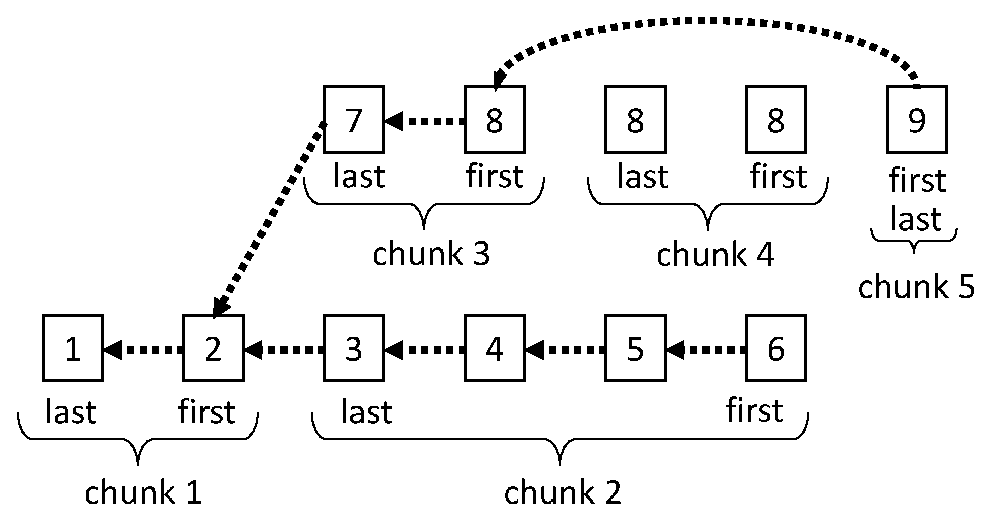
\includegraphics[width=0.6\linewidth]{img/ChunkFullp1.eps}
  \caption{An usage of chunk data structures}
  \label{fig:chunk1}
\end{figure}
There are five chunks in this figure, and several of them are linked together with \texttt{first} element: ``5'' and ``4'', ``4'' and ``3'', ``3'' and ``1'', ``2'' and ``1''. Chunk 4 is empty. Numbers are the identifiers of the corresponding nodes. Empty chunk duplicates node \texttt{first} of its left hand linked node.


%---------------------
\subsubsection{Proof state tree.}
A proof state tree (PST) is a tree structure of the following properties: the root is the original PCF, other nodes are consequent subformulas (with its answer applied and variables renamed). In addition, the nodes contain some system information like step of inference, answer, etc. Thus, the number of the leafs of the PST is the current number of the bases, and at current inference step, a PCF is denoted by the path from the leaf to the PST root. This approach allows us to rollback (backtrack) the inference search process, observe proof states and share references among terms and formulas. If a base is refuted then its structures can be released by deleting the path from corresponding leaf to the nearest branching.

Every node of a PST is a chunk. The growth of the tree is a linking of new chunks with the existing leafs of the tree from the left hand.

PST for the formula from Example \ref{proofexample} is represented in Fig.~\ref{fig:pst}.
PST root is an original PCF $F_1$. Node ``2'' is a  $Q_1$ question consequent $\exists\colon A(a)$, and the path from node ``2'' to the root node corresponds to PCF $F_2$. Nodes ``3'' and ``4'' are corresponding consequents for $Q_4$. The path from node ``3'' to the root node and the path from node ``4'' to the root node correspond to base subformulas for PCF $F_3$. For example, formulas that are denoted by paths ``5''--``1'' and ``3''--``1'' share data that are represented by nodes ``1''--``2''. When base subformula that is represented by path ``3''--``1'' is refuted, we can delete path from node ``3'' to the nearest branching. In this case only node ``3'' is deleted because nodes ``2''--``1'' are still used for representing another base subformulas.
%The lettering in figures should have a height of 2mm (10-point type)
%caption UNDER the figures
\begin{figure}[h]
  %\vspace{0.5cm}
  \centering
  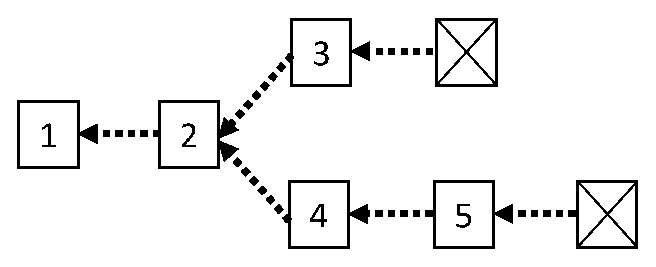
\includegraphics[width=0.4\linewidth]{img/PSTp1.eps}
  \caption{Proof state tree for PCF from Example \ref{proofexample}}
  \label{fig:pst}
\end{figure}

%---------------------
\subsubsection{Data sharing: sharing of base subformulas.}
%------
The PST structure allow to implement the memory data sharing: if base subformulas have common PST paths, their bases share elements of type conditions and sets of questions (Fig.~\ref{fig:datasharing1}).
\begin{figure}[h]
  \vspace{0.5cm}
  \centering
  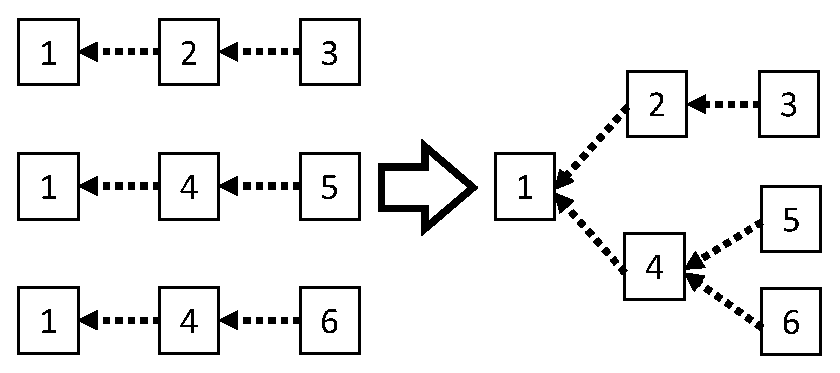
\includegraphics[width=0.4\linewidth]{img/Graphsp1.eps}
  \caption{Memory data sharing}
  \label{fig:datasharing1}
\end{figure}

If a PCF contains a question with disjunctive branching, then its base subformula will be divided into several new base subformulas during searching procedure of the logical inference. The number of new subformulas corresponds to the number of disjunctive subformulas in the consequent of the question. In a straightforward variant of the prover implementation, the sharing will require copying previous state of the original formula more than once; this copying have a linear complexity, and it leads to the redundant expenses of memory and processor time. PST allows us to implement common subbranches sharing instead of copying. Let's consider the following base subformula:
$$\exists: A(a) - \forall x: A(x) - \left\{
\begin{array}{lcl}
 \exists \colon B(x) & - & \forall y: B(y) - \exists\colon\boldsymbol{False}\\
 \exists \colon C(x) & - & \forall y: C(y) - \exists\colon\boldsymbol{False}.
\end{array}
\right. $$
The formula has disjunctive branching and it is deep. PST for the refutation of this base subformula is presented in Fig.~\ref{fig:datasharing2}.
\begin{figure}[h]
  \vspace{0.5cm}
  \centering
  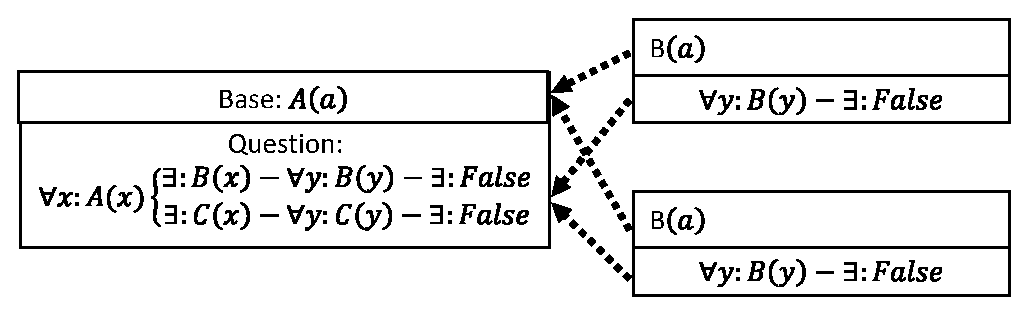
\includegraphics[width=0.82\linewidth]{img/DataSharing2p1.eps}
  \caption{Example of PST for a base subformula refutation}
  \label{fig:datasharing2}
\end{figure}




%====================================================================================
%====================================================================================
\subsection{Lazy instantiation}

According to the Definition~3, the inference rule $\omega$ can be applied if a question $\forall \bar{y}\colon A$ to a base $\exists \bar{x}\colon B$ has an answer $\theta$, such that $\theta$ is a substitution $\bar{y} \rightarrow H^{\infty}$ and $A\theta \subseteq B$. If all the variables in $\bar{y}$ are occurred in $A$, then the search of corresponding elements from $H^{\infty}$ is carried on by the algorithm of subsumption among corresponding base of facts, since the conditions of subsumption of the sets have to be satisfied. If a variable in the $\bar{y}$ is not occurred in $A$ then the variable is called \emph{unconfined variable} and it is not used in a subsumption. However, we need to find a substitution for these variables as well.  Each of the elements of Herbrand universe is a correct substitution for the unconfined variable. This rises a problem related to Herbrand universe. In the general case the universe is an unlimited set, and it is not known what element should be taken as a substitution for the variable.

The main concept of lazy instantiation is as follows. Instead of selecting a concrete element of a Herbrand universum for a substitution of an unconfined variable an {\em unspecified Herbrand element} (UHE) is used temporally. The UHE will be concretized further to a proper term. The result of the concertizing depends on the logical inference strategy. UHE will be instantiated to a ground term, or in some situations, it could remain unbound.

The UHE can be concretized in a term, containing other UHEs. The variant of the concretizing on the each step is chosen according to inference strategies to make refutation possible, e.g. by analyzing a term structure of a question.  The process is organized in a trendy ``lazy'' manner: UHE is instantiate as concrete, as it is enough for answering a question, i.e. instantiation is generally partial, for example UHE for $h$ is concretized to $f(h_1)$, where $h_1$ is a new UHE.

UHE by nature is similar to unconcretized $\forall$-variable in the sense that it is mutable, i.e., it is potentially concretized, however all such changes must be aimed at instantiation of  UHE, i.e. UHE can be substituted only to a term or to other UHE, but not to a variable.

Let's consider an example of the technique application in building a logical inference for the following formula.
\begin{equation*}
  \forall\colon\boldsymbol{True} - \exists\colon\boldsymbol{True} -
  \left\lbrace
  \begin{array}{l}
    \forall x\colon\boldsymbol{True} - \exists\colon A(x) \\
    \forall x\colon A(f(x)) - \exists\colon B(f(x)) \\
    \forall\colon B(f(a)) - \exists\colon \boldsymbol{False}
  \end{array}\right.
\end{equation*}

At the first step there is an answer $\{x \rightarrow h_1\}$ to the first questions, $x$ is an unconfined variable and $h_1$ is an unspecified Herbrand element. After this step atom $A(h_1)$ is added to the base. At the second step there is an answer $\{x \rightarrow h_2\}$ to the second question and $h_1$ is instantiated to $f(h_2)$, after this step $B(f(h_2))$ is added to the base. Finally, at the third step the trivial (empty) answer exists to the third question and $h_2$ is concretized to $a$.

To improve the search efficiency of the strategy, we use two constraints.

%Для стртегии ленивой конкретизации предложено два типа ограничений
\subsubsection{Constraint~1: Limit of concretizations number.}
%Ограничение количества конкретизаций.

%---
Two UHEs are \emph{similar}, if they were generated as the result of a substitution for the same unconfined variable. This situation appears if for a question with unconfined variables a sequence of a similar answers were constructed, such that on every step of the sequence new UHE created as a substitution. The constraint for the similar UHE--concretizations excludes the possibilities of generation of new UHE when it is not necessary. For every UHE a reference to its unconfined variable (that resulted to the USE production) is stored. The set of terms, which concretized an unconfined variable through its UHE, is stored in questions. The engine allows tracking the UHE concretization. If a predefined limit of the concretizations is exceeded then all further concretizations rejected. The limit is chosen by user according to a specific and features of the problem under investigation, or it is denoted as $1$, and increased after an unsuccessfull logical inference, then the inference attempt is repeated.

\subsubsection{Constraint~2: Storing expressions which contain UHE.}
%Сохранение выражений, содержащих НЭЭ

Another UHE--approach to process unconfined variables is based on storing in an UHE original type condition that contained the variable.  Later it could be used as a constrain for possible substitution value from $H^{\infty}$ acceptable to form an answer. This is a form of lazy computation of other form as compared to lazy concretizing, but instead of sequential concretizing the USE instantiates by a term from a set $H^{\infty}$. The installation is stored in UHE. If the UHE can be instantiated in a new value from $H^{\infty}$, it does, and the value also stored in UHE. So we can count values one by one and prohibit repeating.


%====================================================================================
%-----------------k,m,-condition-----------------
\subsection{Strategy of ``$\boldsymbol{k,m}$-constraint"}
An answer to a question is accepted if at some point of the following $k$ steps of its inference a certain condition becomes true at least $m$ times. This strategy is used in the following cases.

\subsubsection{$\boldsymbol{k,m}$--refutation.} An answer to a question with disjunctive branching is accepted if in next $k$ steps at least $m$ generated bases were refuted, otherwise the process restarted with a new answer. This strategy allows us to constrain highly spawning inferences by means of control answering questions with disjunctive branching.

\subsubsection{$\boldsymbol{k}$--unrefutation.}
For a question with disjunctive branching an answer is accepted if during next $k$ steps no refutation for the base subformula was achieved, using the questions without disjunctive branching. This strategy, as it is in the previous variant, reduces growth of a formula due to answering questions with disjunctive branching. If no refutation can be constructed using this strategy, then answering to the questions allowed.

\subsubsection{$\boldsymbol{k,m}$--concretization.}
An answer for a question is accepted if during next $k$ steps at least $m$ UHE are concretized. This strategy is also aimed at limiting a complexity of the formula. Large amounts of additional information and conditions are associated with unconcretized UHE. After an UHE is concretized, the associations are released. As soon we instantiate the UHE as soon we will take advantage of additional memory.

%====================================================================================
%Parallel strategy
\subsection{Strategy of parallel inference}

Let's consider techniques and strategies for parallel implementations of logical inference algorithms in the PCF calculus.

\subsubsection{Independent asynchronous refutation of bases.}
If a question has disjunctive branching then, after we have answered that question, the formula will splits and transforms to the formula with a set of bases according to the set of answered question consequents, i.e. in general case the number of the base subformulas is increasing in every step of logical inference. In addition, the original formalization of a problem in PCF language can contain more than one base subformulas. In order to refute the original PCF formula every base need to be refuted. The refutation of the base subformulas can be processed in parallel in an independent thread. This is possible if the bases are independent from each other, i.e. they don't share $\forall$--variables and UHEs. Bases never share $\forall$--variables because bases don't contain $\forall$--variables at all (by definitions), as they contain only ground terms. However, bases can share the UHEs in case of usage of the lazy concretization strategy. Therefore, this strategy can be applied in case if the lazy concretization strategy is not used. According to features of PCF, the PCF have property called ``OR--parallelism''.

\subsubsection{Parallel answer search.}
In addition to the OR--parallelism, parallel schemes of algorithms to search answers for each questions can be constructed. Since the questions do not share variables, as in previous strategy, the answer search procedure can be performed also in an individual computation thread. In addition, like in the previous strategy, second parallel strategy formulated as follows: each answer search procedure to a question is independent of other questions.

Scheduling threads and process on a cluster nodes must be carried out as usual according to the cluster parameters related to CPU performance and network throughput. For example, implementation of base formula refutation procedures should be bound to a process on a computing node. The same is not true for the second strategy, as is possible to degrade overall inference search efficiency by communication delays. So the refutation process in PCF having no unconfined variables are naturally scaled among cluster nodes and all the processes run independently on each other.

\subsection{Memory management}
Allocation of memory for fixed size records is implemented by means of standard approach, which is similar to \cite{gmemory}. Array of structures is allocated with memory manager of operation system and then converted to freelists. New structures are allocated from the freelists, and released ones are returned back to the freelists. If a list is exhausted a new array is allocated from heap memory if any.

In the prover for each variant of records, own array is allocated and own freelist constructed. The garbage collection is synchronized with garbage collector of the D programming language run time engine.


%=======================================================================
%==========================EXPERIMENTS==================================
%=======================================================================
\section{Experiments}
Testing the developed prover is being performed on problems form TPTP \cite{tptp} library version 5.4.0 (Thousands of Problems for Theorem Provers, www.tptp.org). This library is the de facto standard for testing ATP provers. The type of problems that were chosen are the problems of FOF without equality. Total number of problems is 1221 with rating from 0.0 (very easy) to 1.0 (unresolved). Total number of solved problems is 780. The maximal rating of solved problem is 0.62. The best results among domains presented in the Table~1.

\begin{table}
\caption{Domains}
\begin{tabular}{|p{0.3\linewidth}|p{0.4\linewidth}|p{0.1\linewidth}|}

\hline
\textbf{Domain} & \textbf{No of problems in the domain} & \textbf{Solved} \\
\hline
Geometry (GEO) & 242 & 204 \\
\hline
Management (MGT) & 22 & 22 \\
\hline
Syntactic  (SYN) & 275 & 180 \\
\hline
Semantic Web  (SWB) & 25 & 22 \\
\hline
\end{tabular}
\end{table}

10 hardest problems solved by our prover is presented in the Table~2.
\begin{table}
\caption{Hardest problems solved by our prover}
\begin{tabular}{|p{0.2\linewidth}|p{0.2\linewidth}|p{0.2\linewidth}|p{0.2\linewidth}|}

\hline
\textbf{Problem} & \textbf{Rating} & \textbf{Time (s)} & \textbf{Steps number} \\
\hline
COM008+1 & 0.62 & 1.9 & 33551 \\
\hline
LCL640+1.005 &  0.62 &  0.06 &  821 \\
\hline
LCL656+1.010 &  0.58 &  1.5 &  43 \\
\hline
SWB012+3 &  0.54 &  65.64 &  102428 \\
\hline
SYN353+1 &  0.54 &  0.002 &  33 \\
\hline
SYN548+1 &  0.54 &  0.01 &  15 \\
\hline
SWB020+2 &  0.5 &  0.6 &  618 \\
\hline
LCL666+1.005 &  0.5 &  0.35 &  2592 \\
\hline
KRS235+1 & 0.46 & 5.4 & 24406 \\
\hline
SWB029+3 &  0.38 &  55.27 &  98471 \\
\hline
\end{tabular}
\end{table}

%График...

Prover shown good results for problems, whose formalization in the PCF language contains large conjuncts (type conditions).

\subsection{Translation from TPTP to PCF}
TPTP contains an axiom library, which consists of different files. Formula to be investigated is collected from the files. The collection is performed with special utilities such as \texttt{tptp4X}. The collected subformulas are passed to a translator from TPTP representation to the input language of the prover. The translator is implemented with the \texttt{hotptp-yl-parser-verbose} \cite{TPTPTrans} utility that translates input TPTP--files to abstract syntax trees. Translation component of the utility is generated on the base of syntactic analysis of the current specification of TPTP. Therefore, in each case of the specification refinement, the utility can be automatically updated (recompiled). Using this approach, we are able to adopt our prover to the new input language specification.

The abstract syntax tree is passed to translation component that imports the tree, translates the predicate formula or CNF, performs some reduction of subformulas by applying a set of rules, converts the formulas into the PCF language, performs additional reduction of the PCFs, renames the quantifier variables, and, at the last step, outputs the conversion result as textual representation of the problem in the language of the prover.


\subsection{Example of Formula}
Problem SYN380+1.p from TPTP library in our prover input language has a following form:
\begin{quote}
\texttt{\raggedright\noindent
\{\\
~~e[][]~\{\\
~~~~a[W][big\_r(W,W)]~\{\\
~~~~~~e[][False]~\{\}\};\\
~~~~a[X,Y][]~\{\\
~~~~~~e[][big\_r(X,Y)]~\{\};\\
~~~~~~e[Z][big\_q(Y,X)]~\{\\
~~~~~~~~a[][big\_q(Z,Z)]~\{\\
~~~~~~~~~~e[][False]~\{\}\}\}\}\}\\
\}\\
}
\end{quote}

\subsection{Example of solved problem}
Let us consider COM003+1.p (``The halting problem is undecidable'') problem with 0.33 rating.

The results of solving this problem by our prover and other provers are presented in Table~3.

\begin{table}
\caption{COM003+1.p solving}
\begin{tabular}{|p{0.2\linewidth}|p{0.35\linewidth}|}

\hline
\textbf{Prover} & \textbf{Time (s)} \\
\hline
Our prover & 0.05 \\
\hline
Vampire & 0.01 \\
\hline
iProver & 0.27 \\
\hline
leanCoP & 19.25 \\
\hline
EP & 54.45  \\
\hline
Zenon & 0.08 \\
\hline
\end{tabular}
\end{table}

%Рассмотрим задачу TPTP SYN548+1.

%В языке ПО-формул формализация выглядит следующим образом:

%Рейтинг 0.54. Время решения: 5.8с. Количество шагов: 82764.

%При решении данной задачи использовались стратегии: ленивая конкретизация (ограничение 1), $8$--неопровержимость, $8,1$--конкретизация, разделение данных по базе, агрессивное разделение термов.

%Let's consider problem SYN548+1 from TPTP.
%In PCF language formalization looks like the following:

%Rating is 0.54. Time for solving 5.8s. Number of steps: 82764.

%The lazy concretization (first constraint), $8$--unrefutation, $8,1$--concretization, data sharing in bases.



%==========================================================
\subsection{Comments on strategies}

%=============================
\subsubsection{Lazy concretization.}
Lazy concretization strategy allows one in most cases to find a substitution for an unconfined variable in acceptable time as compared to the sequential enumeration of Herbrand universum. The constraints are the most valuable part of this strategy, which allow to decrease the number of steps of logical inference in comparison to the unconstrained strategy. The decrease of the number of steps leads to a decrease of the problem solving time. Application of the constraint~1 is the best way of the inference time reduction in the case when a formula has questions with disjunctive branching and the constraint~2 in case if the formula contains no questions without disjunctive branching.


%=============================
\subsubsection{$k,m$--condition.}
The efficiency of this strategy reveals in the problems with disjunctive branching. In all cases of acceptable application of this strategy and correctly chosen parameters, the noticeable improvement is achieved.
%===========================
\subsubsection{Parallel stratgies.}
The important quality of parallel schemes of algorithms is their scalability, i.e., the performance improvement respect to increase of the number of computational nodes (CNs). That’s why the main characteristic of the prover productivity is not the time of execution of the program, but the ratio of program execution time in parallel mode on a given number of CNs to the program execution time on a single CN. The ratio is accounted for various number of CNs.

Experiments were carried out on the logical problems which PCF--formalizations have necessary properties for the parallel strategies: disjunctive branching, large number of questions, large conjuncts in questions. In Fig.~\ref{fig:parallel} the results of experiments are shown.

\begin{figure}[h]
  %\vspace{0.5cm}
  \centering
  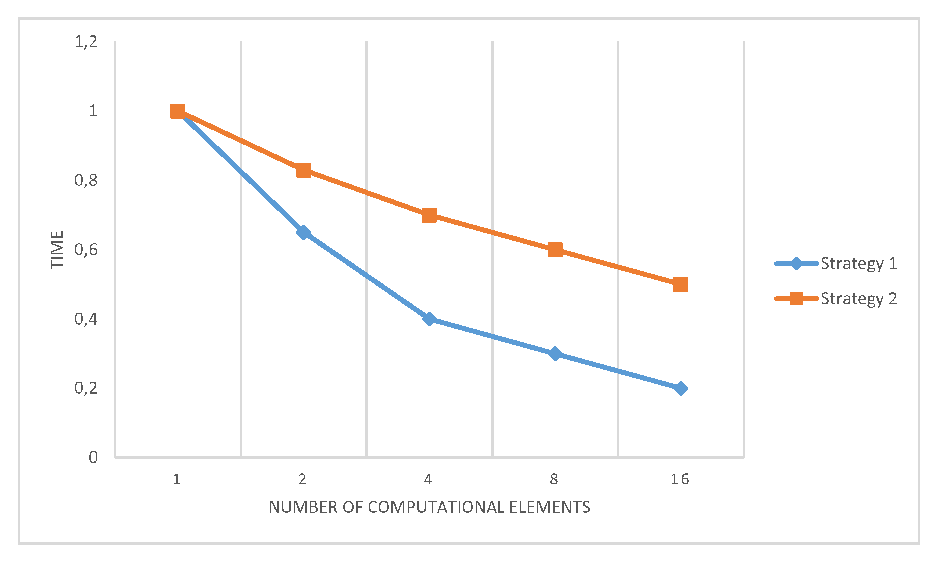
\includegraphics[width=0.8\linewidth]{img/Parallel.eps}
  \caption{Results of parallel strategies testing}
  \label{fig:parallel}
\end{figure}




%=======================================================================
%==========================CONCLUSION===================================
%=======================================================================
\section*{Conclusion}
In this paper, we presented the results of the positively constructed formulas (PCF) calculus investigation in the context of the automatic theorem proving. The main result is a prover program implemented based on the PCF calculus. Several logical inference strategies were devised, adopted from other papers and implemented in this prover: memory sharing, lazy concretization, $k,m$--condition, parallel strategies. A special global data structure (proof state tree) has been developed. Most of the strategies are implemented on the base of the structure.

Testing our prover has been carried out on problems from TPTP library. Testing has shown that the PCF calculus is suitable for automated theorem proving and some problems are solved more efficiently than other provers. The classes of problems, which are the most suitable for our system, are described.

Further investigations aimed at implementation of a productive logical inference engine with equality and with indexing techniques, for example, substitution tree indexing \cite{subtree}. The application of this prover for solving the problems of dynamic systems control will be investigated also.



%=======================================================================
%==========================BIBLIOGRAPHY=================================
%=======================================================================
\begin{thebibliography}{4}

\bibitem{DPL2} Alexandrescu, A. The D Programming Language. -- Addison-Wesley Professional, 2010. -- 460p.

\bibitem{DPL1} Armstrong, J. D Programming Language. URL: http://www.digitalmars.com/d/.

\bibitem{Erlang1} Armstrong, J. Programming Erlang.  -- The Pragmatic Programmers, 2007. -- 519p.

\bibitem{TPTPTrans} Gelder, A.V. TPTPparser utility. 2006. URL: http://users.soe.ucsc.edu/\~{}avg/TPTPparser/.

\bibitem{gmemory} GLIB: Memory Slices. URL: http://developer.gnome.org/glib/2.34/glib-Memory-Slices.html.

\bibitem{subtree} Graf, P. Substitution Tree Indexing // Proceedings of the 6th International Conference on Rewriting Techniques and Applications. 1995. pp.~117--131.

%\bibitem{HAR} Robinson, A., Voronkov, A. (eds.) Handbook of Automated Reasoning. -- MIT Press, Cambridge, 2001. -- 2150p.

\bibitem{tptp} Sutcliffe, G. The TPTP Problem Library and Associated Infrastructure: The FOF and CNF Parts, v3.5.0 // Journal of Automated Reasoning. V43, N4, pp.337--362.

\bibitem{SNV1990} Vassilyev, S.N.: Machine Synthesis of Mathematical Theorems. The Journal of Logic programming, V.9, No.2--3, pp. 235--266 (1990)

\bibitem{ICDS2000} Vassilyev, S.N., Zherlov, A.K., Fedunov, E.A.,
Fedosov, B.E.: Intelligent Control of Dynamic Systems. Moscow: Fizmatlit (2000)(in Russian)

\end{thebibliography}




\end{document}

%%% Local Variables:
%%% mode: latex
%%% TeX-master: t
%%% End:
